% =====================================================================
%  Framework architecture diagram for the Dewberry deck.
%  A slide-oriented redrawing of Fig. 1 of
%    Massoudieh (2023), Environmental Modelling and Software 164, 105707
%    "A simplified UML class diagram of the OpenHydroQual modeling framework"
%
%  Differences from the paper figure, all for legibility on a projector:
%    - colour coding: core classes blue, component types teal, plugins and
%      the estimation engines rust
%    - the paper's six dashed calibration arrows are collapsed into one
%      labelled feedback loop
%    - sentence case instead of all caps
%
%  Build:  pdflatex fig_framework.tex && cp fig_framework.pdf figures/N8_framework.pdf
% =====================================================================
\documentclass[border=4pt]{standalone}
\usepackage[T1]{fontenc}
\usepackage{helvet}
\renewcommand\familydefault{\sfdefault}
\usepackage{tikz}
\usetikzlibrary{arrows.meta,positioning,shapes.multipart,fit,backgrounds,calc}

\definecolor{ohqblue}{HTML}{1F5C8B}
\definecolor{ohqteal}{HTML}{2A9D8F}
\definecolor{ohqrust}{HTML}{E76F51}
\definecolor{ohqgrey}{HTML}{6B7280}
\definecolor{bandfill}{HTML}{EDF1F4}
\definecolor{chemfill}{HTML}{E3E9EE}

\begin{document}
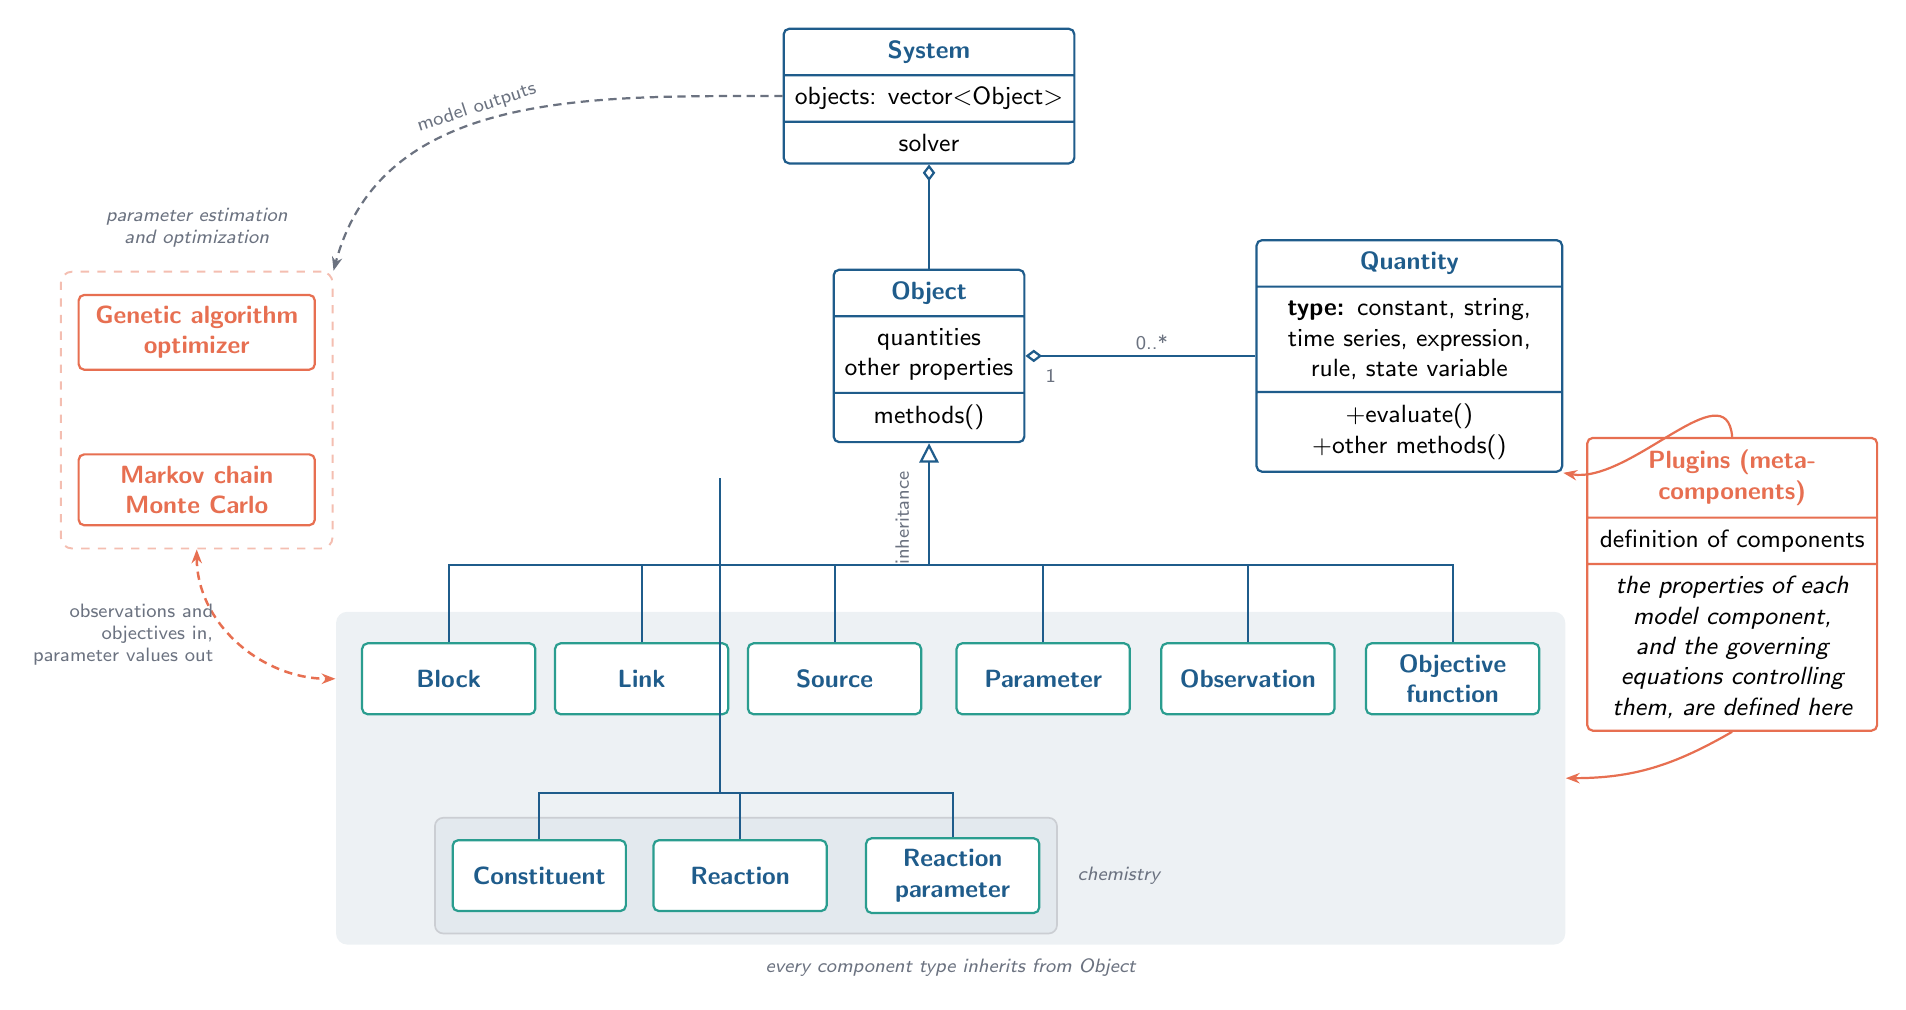
\begin{tikzpicture}[
  font=\sffamily,
  cls/.style={
    draw=ohqblue, line width=0.8pt, fill=white, rounded corners=2pt,
    rectangle split, rectangle split part align=center,
    align=center, inner sep=4pt, font=\small},
  leaf/.style={
    draw=ohqteal, line width=0.8pt, fill=white, rounded corners=2pt,
    align=center, inner sep=4pt, font=\small\bfseries,
    text=ohqblue, minimum height=9mm, minimum width=22mm},
  aux/.style={
    draw=ohqrust, line width=0.8pt, fill=white, rounded corners=2pt,
    align=center, inner sep=4pt, font=\small\bfseries,
    text=ohqrust, minimum height=9mm, minimum width=30mm},
  owns/.style={{Diamond[open, length=6pt, width=4.5pt]}-, ohqblue, line width=0.8pt},
  inherit/.style={-{Triangle[open, length=7pt, width=7pt]}, ohqblue, line width=0.8pt},
  spinepart/.style={ohqblue, line width=0.7pt},
  loop/.style={{Stealth[length=5pt]}-{Stealth[length=5pt]}, ohqrust,
               line width=0.9pt, dashed, dash pattern=on 3pt off 2pt},
  feed/.style={-{Stealth[length=5pt]}, ohqgrey, line width=0.8pt,
               dashed, dash pattern=on 3pt off 2pt},
  defines/.style={-{Stealth[length=5pt]}, ohqrust, line width=0.8pt},
  lbl/.style={font=\scriptsize, text=ohqgrey, inner sep=2pt},
  note/.style={font=\scriptsize\itshape, text=ohqgrey, align=center},
]

% ================= core classes ====================================
\node[cls, rectangle split parts=3] (system) at (0,0)
  {\textbf{\textcolor{ohqblue}{System}}
   \nodepart{two} objects: vector\textless Object\textgreater
   \nodepart{three} solver};

\node[cls, rectangle split parts=3] (object) at (0,-3.3)
  {\textbf{\textcolor{ohqblue}{Object}}
   \nodepart{two} quantities \\ other properties
   \nodepart{three} methods()};

\node[cls, rectangle split parts=3, text width=36mm] (quantity) at (6.1,-3.3)
  {\textbf{\textcolor{ohqblue}{Quantity}}
   \nodepart{two}\raggedright \textbf{type:} constant, string, time
     series, expression, rule, state variable
   \nodepart{three} +evaluate() \\ +other methods()};

% ================= component types (inherit from Object) ===========
\node[leaf] (block)  at (-6.10,-7.4) {Block};
\node[leaf] (link)   at (-3.65,-7.4) {Link};
\node[leaf] (source) at (-1.20,-7.4) {Source};
\node[leaf] (param)  at ( 1.45,-7.4) {Parameter};
\node[leaf] (obs)    at ( 4.05,-7.4) {Observation};
\node[leaf] (objf)   at ( 6.65,-7.4) {Objective\\function};

\node[leaf] (const)  at (-4.95,-9.9) {Constituent};
\node[leaf] (rxn)    at (-2.40,-9.9) {Reaction};
\node[leaf] (rxnpar) at ( 0.30,-9.9) {Reaction\\parameter};

\begin{scope}[on background layer]
  \node[fill=bandfill, rounded corners=4pt,
        fit=(block)(objf)(const)(rxnpar),
        inner xsep=9pt, inner ysep=11pt] (band) {};
  \node[fill=chemfill, draw=ohqgrey!35, line width=0.6pt, rounded corners=3pt,
        fit=(const)(rxnpar), inner xsep=6pt, inner ysep=7pt] (chem) {};
\end{scope}
\node[lbl, anchor=north] at ([shift={(0,-3pt)}]band.south)
  {\itshape every component type inherits from Object};
\node[lbl, anchor=west] at ([shift={(5pt,0)}]chem.east)
  {\itshape chemistry};

% ================= plugins =========================================
\node[cls, rectangle split parts=3, text width=34mm, draw=ohqrust] (plug) at (10.2,-6.2)
  {\textbf{\textcolor{ohqrust}{Plugins (meta-components)}}
   \nodepart{two} definition of components
   \nodepart{three}\itshape the properties of each model component, and the
     governing equations controlling them, are defined here};

% ================= calibration engines =============================
\node[aux] (ga)   at (-9.3,-3.0) {Genetic algorithm\\optimizer};
\node[aux] (mcmc) at (-9.3,-5.0) {Markov chain\\Monte Carlo};
\begin{scope}[on background layer]
  \node[draw=ohqrust!45, dashed, line width=0.7pt, rounded corners=4pt,
        fit=(ga)(mcmc), inner xsep=6pt, inner ysep=8pt] (engines) {};
\end{scope}
\node[note, anchor=south, text width=36mm] at ([shift={(0,5pt)}]engines.north)
  {parameter estimation\\and optimization};

% ================= relations =======================================
% composition: the diamond sits on the owning class
\draw[owns] (system.south) -- (object.north);
\draw[owns] (object.east) -- node[lbl, above, pos=0.55] {0..*} (quantity.west);
\node[lbl] at ($(object.east)+(0.32,-0.26)$) {1};

% inheritance spine
\coordinate (spine) at ($(object.south)+(0,-1.55)$);
\draw[inherit] (spine) -- (object.south);
\node[lbl, rotate=90, anchor=south] at ($(object.south)+(-0.18,-0.95)$) {inheritance};
\foreach \n in {block,link,source,param,obs,objf}
  \draw[spinepart] (\n.north) |- (spine);
\coordinate (chemspine) at ($(chem.north)+(0,0.30)$);
\foreach \n in {const,rxn,rxnpar}
  \draw[spinepart] (\n.north) |- (chemspine);
% up the clear channel between Link and Source to the main inheritance spine
\draw[spinepart] (-2.65,-8.85) -- (-2.65,{-4.85});

% plugins define both the component types and the quantity vocabulary
\draw[defines] (plug.north) to[out=95, in=-10] (quantity.south east);
\draw[defines] (plug.south) to[out=-150, in=0] (band.east);

% model outputs feed the estimation engines; they set parameters in return
\draw[feed] (system.west) to[out=180, in=75]
  node[lbl, above, sloped, pos=0.55] {model outputs} (engines.north east);
\draw[loop] (engines.south) to[out=-90, in=180]
  node[lbl, pos=0.45, anchor=east, align=right, xshift=-4pt]
  {observations and\\objectives in,\\parameter values out}
  (band.west |- block.west);

\end{tikzpicture}
\end{document}
